\documentclass[../Matematyka.tex]{subfiles}

\begin{document}
\section{Teoria mnogości}

\subsection{Działania na zbiorach}

\subsubsection*{Suma}
\[C = A \cup B\]

\begin{figure}[H]
    \centering
    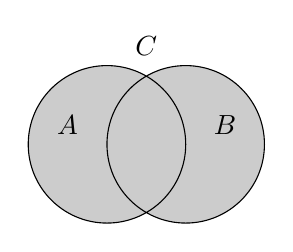
\begin{tikzpicture}[fill=black!20]
        \fill (-0.5,0) circle (1);
        \fill (0.5,0) circle (1);
        % outline
        \draw (-0.5,0) circle (1) (-1,0)  node [text=black,above] {$A$}
        (0.5,0) circle (1) (1,0)  node [text=black,above] {$B$}
        (0,1)  node [text=black,above] {$C$};
    \end{tikzpicture}
\end{figure}

\subsubsection*{Iloczyn}
\[D = A \cap B\]

\begin{figure}[H]
    \centering
    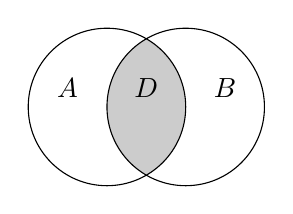
\begin{tikzpicture}[fill=black!20]
        \begin{scope}[even odd rule]
            \clip (-1.5,-1) rectangle (1.5,1)
            (-0.5,0) circle (1)
            (0.5,0) circle (1);
            \fill (-0.5,0) circle (1);
            \fill (0.5,0) circle (1);
        \end{scope}
        % outline
        \draw (-0.5,0) circle (1) (-1,0)  node [text=black,above] {$A$}
        (0.5,0) circle (1) (1,0)  node [text=black,above] {$B$}
        (0,0)  node [text=black,above] {$D$};
    \end{tikzpicture}
\end{figure}

\subsubsection*{Różnica}
\[E = A \setminus B\]

\begin{figure}[H]
    \centering
    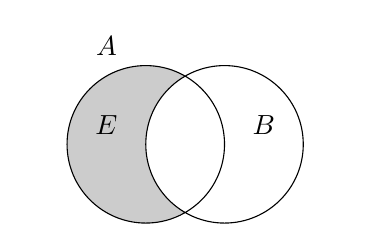
\begin{tikzpicture}[fill=black!20]
        \begin{scope}
            \clip (-2,-1) rectangle (2,1)
            (0.5,0) circle (1);
            \fill (-0.5,0) circle (1);
        \end{scope}
        % outline
        \draw (-0.5,0) circle (1) (-1,1)  node [text=black,above] {$A$}
        (-1,0)  node [text=black,above] {$E$}
        (0.5,0) circle (1) (1,0)  node [text=black,above] {$B$};
    \end{tikzpicture}
\end{figure}

\subsubsection*{Dopełnienie zbioru}
\[A` = X \setminus A\]

\begin{figure}[H]
    \centering
    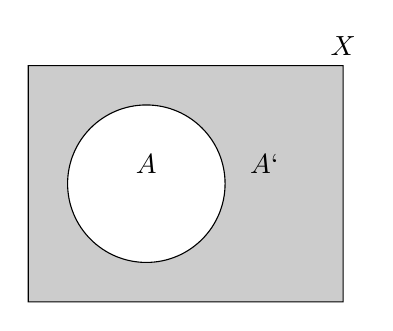
\begin{tikzpicture}[fill=black!20]
        \begin{scope}
            \clip (-0.5,0) circle (1)
            (-2,-1.5) rectangle (2,1.5);
            \fill (-2,-1.5) rectangle (2,1.5);
        \end{scope}
        % outline
        \draw (-0.5,0) circle (1) (-0.5,0)  node [text=black,above] {$A$}
        (-2,-1.5) rectangle (2,1.5) node [text=black,above] {$X$}
        (1,0) node [text=black,above] {$A`$};
    \end{tikzpicture}
\end{figure}

\newpage
\subsection{Iloczyn kartezjański}
\[A \times B = \{(a, b) : a \in A \; \text{i} \; b \in B\}\]

\[A = \{a, b, c\} \qquad B = \{1, 2\}\]
\[A \times B = \{(a,1)(a,2)(b,1)(b,2)(c,1)(c,2)\}\]

Oznaczenie: \(|X|\) - ilość elementów

Tw. \(|A \times B| = |A| \cdot |B|\)

\(\mathbb{R}\) - zbiór liczb rzeczywistych (prosta liczbowa)\par
\(\mathbb{R}^2 = \mathbb{R} \times \mathbb{R} = \{(x,y) : x \in \mathbb{R} \; \text{i} \; y \in \mathbb{R}\}\) - płaszczyzna\par
\(\mathbb{R}^n \) - przestrzeń \(n\) wymiarowa
\end{document}